% !TeX root = thesis.tex
\chapter{Results and Discussion}
\label{chap:Results}
\section{Introduction}

This chapter presents and discusses the results obtained from the dimensionality reduction and compression methods applied to structured clinical data. It summarises the baseline characteristics of the dataset, the effects of feature selection and dimensionality reduction, and the performance of different file formats during transfer from the clinic-side computer to the university server. It also examines how well the methods preserved the recorded information and the trade-offs between data size, processing time and transfer efficiency.

\noindent The five figures in this chapter were drawn from the archived experiment summaries. The plotting script (\path{Codes/generate_figures.R}) and its aggregate input accompany the manuscript.

\section{Dataset and Experimental Arrangement}\label{dataset-and-experimental-arrangement}

The study used a structured sepsis dataset obtained from Training Set A of the PhysioNet/Computing in Cardiology Challenge 2019 \citep{Reyna2019}. The dataset contained 20,336 patients, 790,215 hourly records and 43 columns. Data transfer was evaluated between a sending workstation representing a clinical data source and a university computing server at KNUST. The main experiment used authenticated SCP over SSH and remote SHA-256 checks. Two further experiments compared SCP and rsync over this route, first on prepared archives and then on the five files retained from Phase Two. The experiments examined feature selection, dimensionality reduction, compression and transfer performance.


\section{Phase One: Baseline Data
	Profiling}\label{phase-one-baseline-data-profiling}

Baseline profiling showed an overall missing-cell proportion of 65.05\%. The source CSV occupied 75.69 MB, while its loaded DataFrame required approximately 277.37 MB of memory. Data loading took 3.45 s, while the profile calculations required 11.06 s, giving a combined duration of 14.51 s.
Pairwise-complete Pearson
correlations were calculated for the numerical variables using an
absolute-correlation threshold of 0.95. Four of the 861 assessed pairs
exceeded this threshold, and no exactly duplicate column groups were
identified. The correlation results describe statistical redundancy in
the observed data; they were not used to remove variables automatically.

\begin{longtable}[]{@{}lll@{}}
	\caption{Selected missingness and cardinality results.}\label{tab:chapter4-1}\\
	\toprule\noalign{}
	\textbf{Variable} & \textbf{Missing rows (\%)} & \textbf{Observed distinct values} \\
	\midrule\noalign{}
	\endfirsthead
	\toprule\noalign{}
	\textbf{Variable} & \textbf{Missing rows (\%)} & \textbf{Observed distinct values} \\
	\midrule\noalign{}
	\endhead
	\bottomrule\noalign{}
	\endlastfoot
	HR & 7.74 & 333 \\
	O2Sat & 12.03 & 143 \\
	Temp & 66.22 & 597 \\
	Lactate & 96.57 & 351 \\
	Bilirubin\_direct & 99.85 & 139 \\
	TroponinI & 99.88 & 289 \\
	EtCO2 & 100.00 & 0 \\
\end{longtable}

The distribution of missing values was highly uneven. Heart rate and
oxygen saturation were present in most hourly records, whereas Lactate,
Bilirubin\_direct and TroponinI were observed relatively infrequently.
No values were recorded for EtCO2. These differences matter for
dimensionality reduction because a high missingness percentage does not
mean that the available measurements are uninformative. Removing a
sparse laboratory variable eliminates every observation recorded for
that variable, even though its contribution to the serialised file size
may be limited.

\begin{longtable}[]{@{}lll@{}}
	\caption{Pearson correlation pairs exceeding the specified threshold.}\label{tab:chapter4-2}\\
	\toprule\noalign{}
	\textbf{Variable pair} & \textbf{Pearson r} & \textbf{Paired rows} \\
	\midrule\noalign{}
	\endfirsthead
	\toprule\noalign{}
	\textbf{Variable pair} & \textbf{Pearson r} & \textbf{Paired rows} \\
	\midrule\noalign{}
	\endhead
	\bottomrule\noalign{}
	\endlastfoot
	Unit1 / Unit2 & -1.0000 & 404,050 \\
	time / ICULOS & 0.9905 & 790,215 \\
	Bilirubin\_direct / Bilirubin\_total & 0.9621 & 892 \\
	Hct / Hgb & 0.9620 & 68,504 \\
\end{longtable}

The correlation between Unit1 and Unit2 was -1.0000, consistent with
their mutually exclusive coding in the observed records. Time and ICULOS
were strongly positively associated (r = 0.9905). Correlations were also
observed between Bilirubin\_direct and Bilirubin\_total (r = 0.9621),
and between Hct and Hgb (r = 0.9620). The bilirubin correlation was
based on 892 paired records, considerably fewer than the other reported
pairs. Consequently, interpretation of its strength must take the
available paired observations into account. These relationships identify
possible statistical overlap, but do not by themselves establish which
clinical variables may be omitted without affecting future analyses.

\section{Phase Two: Baseline Compression and Network
	Transfer}\label{phase-two-baseline-compression-and-network-transfer}

Baseline transfer performance was evaluated for the original CSV, a
standardised rewritten CSV, gzip-compressed CSV at level 6, Parquet, and
Zstandard-compressed CSV at level 3. File preparation and SSH/SCP
delivery were timed separately. Packaging was measured ten times for
each representation. Network transfer was repeated up to ten times where
the first successful transfer required no more than ten seconds;
otherwise, one successful transfer was recorded. The resulting sample
sizes are shown in Table~\ref{tab:chapter4-3}. The SCP measurements exclude the
separately timed remote checksum-verification operation. The paired comparison below uses the same five files. Section~\ref{sec:paired-results} examines the distinct question of delivering prepared archives.

\begin{longtable}[]{@{}
		>{\raggedright\arraybackslash}p{\dimexpr 0.16\textwidth - 2\tabcolsep\relax}
		>{\raggedright\arraybackslash}p{\dimexpr 0.1429\textwidth - 2\tabcolsep\relax}
		>{\raggedright\arraybackslash}p{\dimexpr 0.1429\textwidth - 2\tabcolsep\relax}
		>{\raggedright\arraybackslash}p{\dimexpr 0.1429\textwidth - 2\tabcolsep\relax}
		>{\raggedright\arraybackslash}p{\dimexpr 0.1429\textwidth - 2\tabcolsep\relax}
		>{\raggedright\arraybackslash}p{\dimexpr 0.1429\textwidth - 2\tabcolsep\relax}
		>{\raggedright\arraybackslash}p{\dimexpr 0.1258\textwidth - 2\tabcolsep\relax}@{}}
	\caption{Baseline size and timing results (means; decimal MB).}\label{tab:chapter4-3}\\
	\toprule\noalign{}
	\textbf{Format} & \textbf{Size (MB)} & \textbf{Saved (\%)} & \textbf{Prep (s)} & \textbf{SCP (s)} & \textbf{Total (s)} & \textbf{Trials} \\
	\midrule\noalign{}
	\endfirsthead
	\toprule\noalign{}
	\textbf{Format} & \textbf{Size (MB)} & \textbf{Saved (\%)} & \textbf{Prep (s)} & \textbf{SCP (s)} & \textbf{Total (s)} & \textbf{Trials} \\
	\midrule\noalign{}
	\endhead
	\bottomrule\noalign{}
	\endlastfoot
	Source CSV & 75.69 & 0.00 & 0.00 & 32.42 & 32.42 & 1 \\
	Rewritten CSV & 77.55 & -2.46 & 18.47 & 36.48 & 54.95 & 1 \\
	CSV + gzip & 14.57 & 80.75 & 21.92 & 9.09 & 31.00 & 10 \\
	Parquet & 9.17 & 87.89 & 0.61 & 7.72 & 8.34 & 10 \\
	CSV + Zstd & 14.67 & 80.62 & 17.60 & 7.97 & 25.57 & 10 \\
\end{longtable}

\begin{figure}
	\centering
	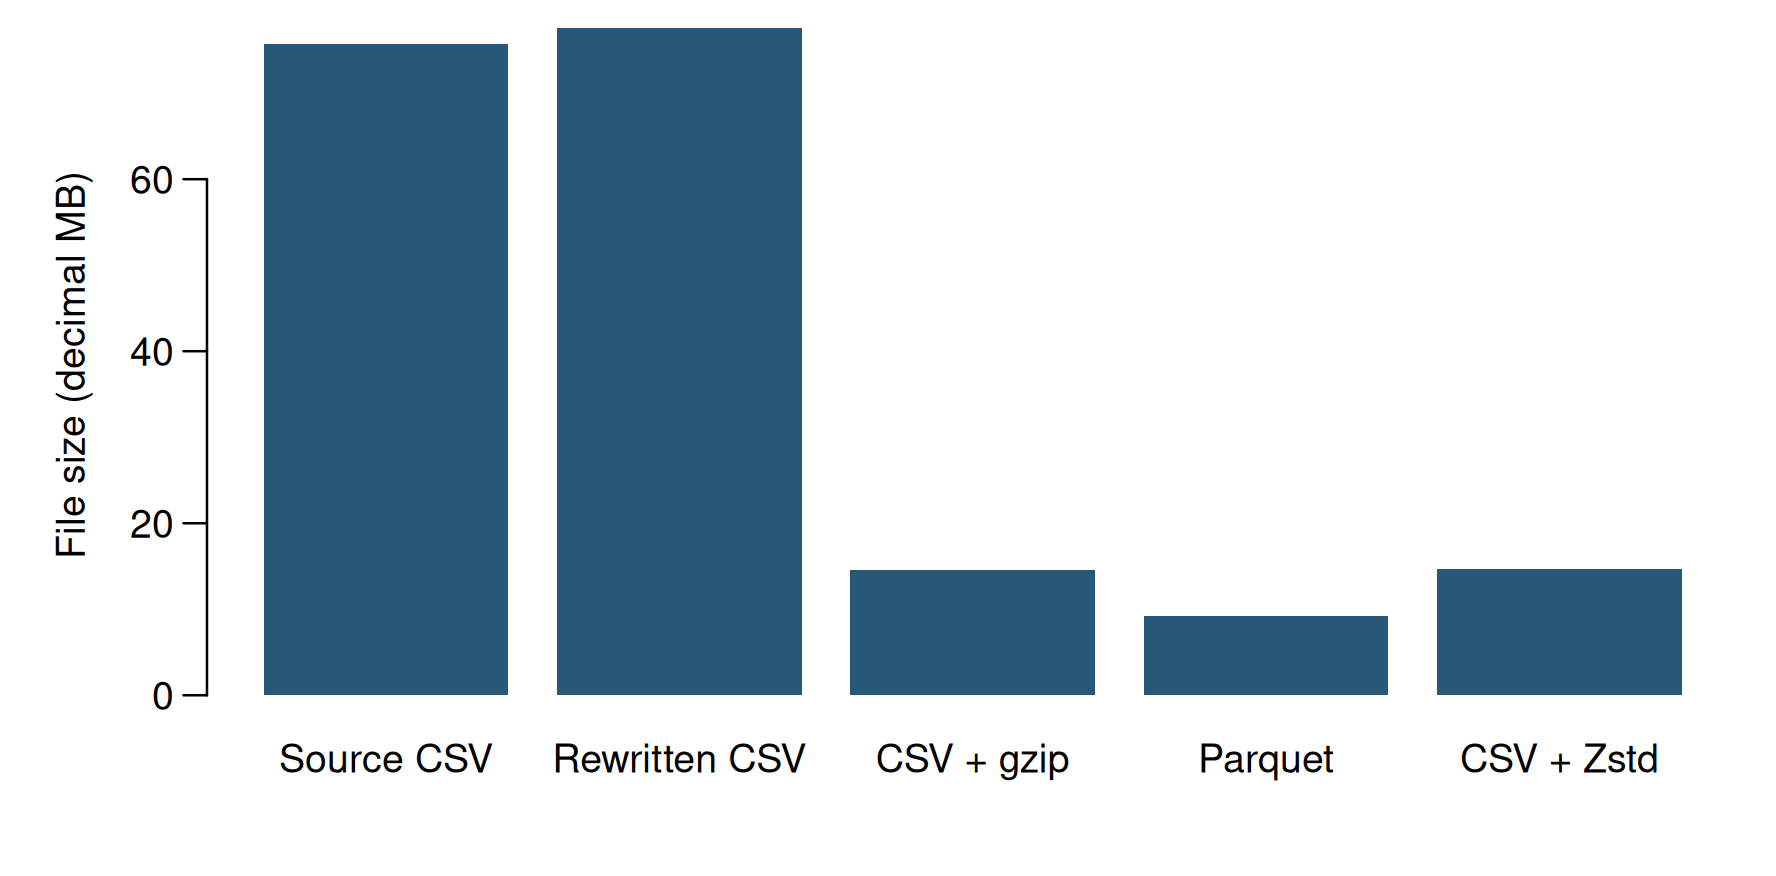
\includegraphics[width=0.84\linewidth,height=0.27\textheight,keepaspectratio]{images/baseline_sizes.png}
	\caption{Baseline representation sizes in decimal megabytes.}\label{fig:chapter4-1}
\end{figure}

\begin{figure}
	\centering
	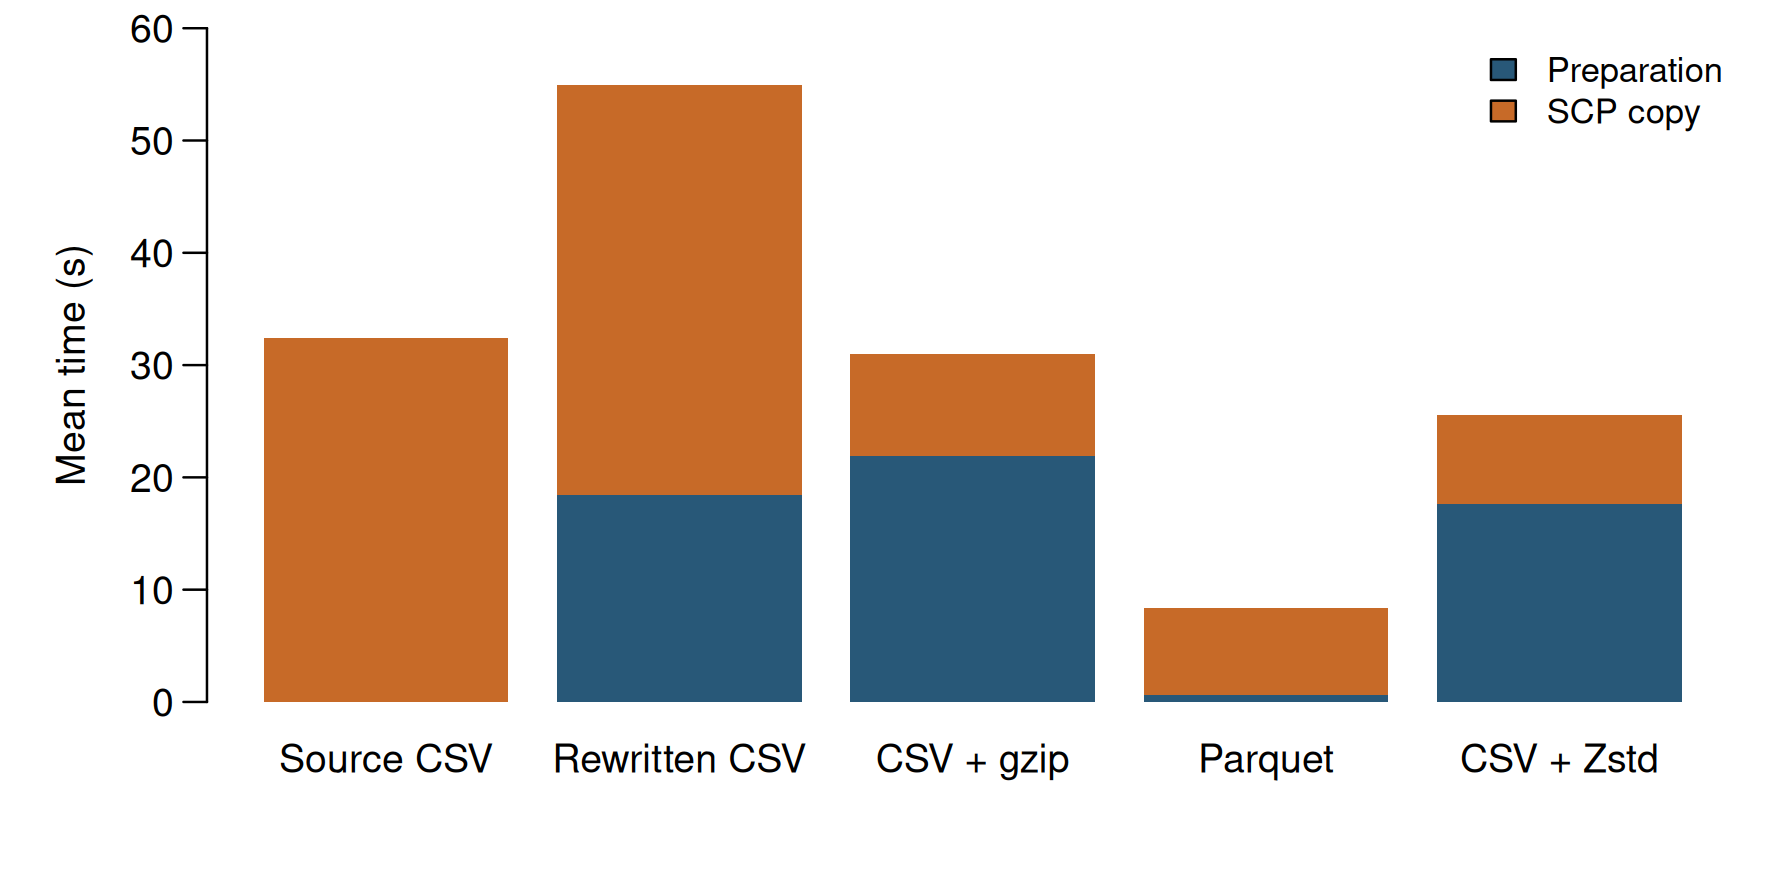
\includegraphics[width=0.84\linewidth,height=0.27\textheight,keepaspectratio]{images/baseline_times.png}
	\caption{Mean packaging and SCP times for the baseline formats. The total excludes verification.}\label{fig:chapter4-2}
\end{figure}

Parquet occupied 9.17 MB, a reduction of 87.89\%
relative to the original file, compared with 14.57 MB for gzip
and 14.67 MB for Zstandard. Its mean measured SCP time was
7.72 s and mean packaging time was 0.61 s, resulting
in an additive packaging-and-transfer estimate of 8.34 s. The
corresponding additive estimates were 31.00 s for gzip and
25.57 s for Zstandard. Rewriting the original CSV increased
file size by about 2.46\%. These results support considering
the cost of producing a compressed representation in addition to
the number of bytes it saves.

The difference in file size was reflected in the observed transfer
durations, although network timing did not vary in direct proportion to
payload size. The source CSV and rewritten CSV each had one observed
transfer, whereas the compressed alternatives had ten, making the former
timings less representative of changing network conditions. In the
separate baseline TOPSIS comparison of the three compressed
alternatives, Parquet obtained the highest relative score (1.000),
followed by Zstandard (0.221) and gzip (0.001). These rankings apply
only to the criteria and normalisation used in the baseline comparison.

\noindent The baseline size and preparation measurements could be reused for a second question. Would the order of the formats change if the same files were sent by rsync?

\subsection{SCP and rsync on the five baseline files}
\noindent All 40 transfers to KNUST passed remote SHA-256 verification on the first attempt. Table~\ref{tab:phase2-paired} gives the results for the four matched pairs per file. The two difference columns were calculated within each block before taking the median. A negative difference means that rsync finished sooner.

\begin{table}[htbp]
\centering
\caption{Direct transfers of the Phase Two files to KNUST. All times are in seconds.}\label{tab:phase2-paired}
\begin{tabular}{@{}lrrrr@{}}
\toprule
 & \multicolumn{2}{c}{Median copy time} & \multicolumn{2}{c}{Median paired difference} \\
\cmidrule(lr){2-3}\cmidrule(l){4-5}
File & SCP & rsync & Copy & Verified delivery \\
\midrule
Source CSV    & 70.59 & 92.77 & $-12.94$ & $-16.35$ \\
Rewritten CSV & 73.48 & 81.49 & $+7.24$  & $+6.73$ \\
gzip          & 27.77 & 26.12 & $-1.65$  & $-3.68$ \\
Parquet       & 16.30 & 16.17 & $-0.13$  & $-2.32$ \\
Zstandard     & 23.11 & 21.29 & $+0.19$  & $-0.27$ \\
\bottomrule
\end{tabular}
\end{table}

\noindent The source CSV illustrates the value of pairing. Rsync copied it sooner in three blocks, by 9.81 to 19.14 seconds, while SCP finished 84.72 seconds sooner in the other block. This variation explains why the two separate medians give a different impression from the within-block comparison. For the rewritten CSV, SCP copied the file sooner in three blocks. For each compressed format, each transport was quicker in two of the four copies. Parquet had the shortest median copy time with either transport.

\noindent The paired Phase Two TOPSIS analysis also placed Parquet first under both transports. With equal weights for size reduction, mean packaging time and mean copy time, the rsync scores were 1.000 for Parquet, 0.264 for Zstandard and 0.001 for gzip. The corresponding SCP scores were 1.000, 0.284 and 0.001. Parquet combined the greatest size reduction and shortest preparation time with the shortest mean copy time in each comparison. A score of 1.000 therefore identifies the best observed combination of these criteria within each transport. The scores do not measure how much faster one transport is than the other.

\section{Phase Three: Feature
	Selection}\label{phase-three-feature-selection}

Feature selection was evaluated at missingness thresholds of 80\%, 90\%
and 95\%, using both missingness-only rules and corresponding
configurations that retained additional variables under patient-coverage
and clinical-protection rules. A configuration without a missingness
threshold provided a further comparison. Forty predictor columns were
considered, while patient\_id, time and SepsisLabel served as structural
fields. Constant columns and exact duplicates were assessed, and strong
correlations were flagged for consideration. The procedures were applied
to the complete dataset because the purpose was to assess data
representation and transfer rather than to train a predictive model.

\begin{longtable}[]{@{}
		>{\raggedright\arraybackslash}p{\dimexpr 0.253\textwidth - 2\tabcolsep\relax}
		>{\raggedright\arraybackslash}p{\dimexpr 0.11\textwidth - 2\tabcolsep\relax}
		>{\raggedright\arraybackslash}p{\dimexpr 0.167\textwidth - 2\tabcolsep\relax}
		>{\raggedright\arraybackslash}p{\dimexpr 0.17\textwidth - 2\tabcolsep\relax}
		>{\raggedright\arraybackslash}p{\dimexpr 0.30\textwidth - 2\tabcolsep\relax}@{}}
	\caption{Feature selection and standardised serialised output sizes.}\label{tab:chapter4-4}\\
	\toprule\noalign{}
	\textbf{Configuration} & \textbf{Kept} & \textbf{Removed (\%)} & \textbf{Selected CSV MB} & \textbf{Reduction vs rewritten CSV (\%)} \\
	\midrule\noalign{}
	\endfirsthead
	\toprule\noalign{}
	\textbf{Configuration} & \textbf{Kept} & \textbf{Removed (\%)} & \textbf{Selected CSV MB} & \textbf{Reduction vs rewritten CSV (\%)} \\
	\midrule\noalign{}
	\endhead
	\bottomrule\noalign{}
	\endlastfoot
	00 no missingness filter & 39 & 2.5 & 76.76 & 1.02 \\
	80 missingness & 13 & 67.5 & 51.17 & 34.02 \\
	80 clinical review & 28 & 30.0 & 66.48 & 14.28 \\
	90 missingness & 19 & 52.5 & 57.99 & 25.22 \\
	90 clinical review & 31 & 22.5 & 69.84 & 9.95 \\
	95 missingness & 29 & 27.5 & 68.18 & 12.09 \\
	95 clinical review & 32 & 20.0 & 70.90 & 8.57 \\
\end{longtable}

\begin{figure}[H]
	\centering
	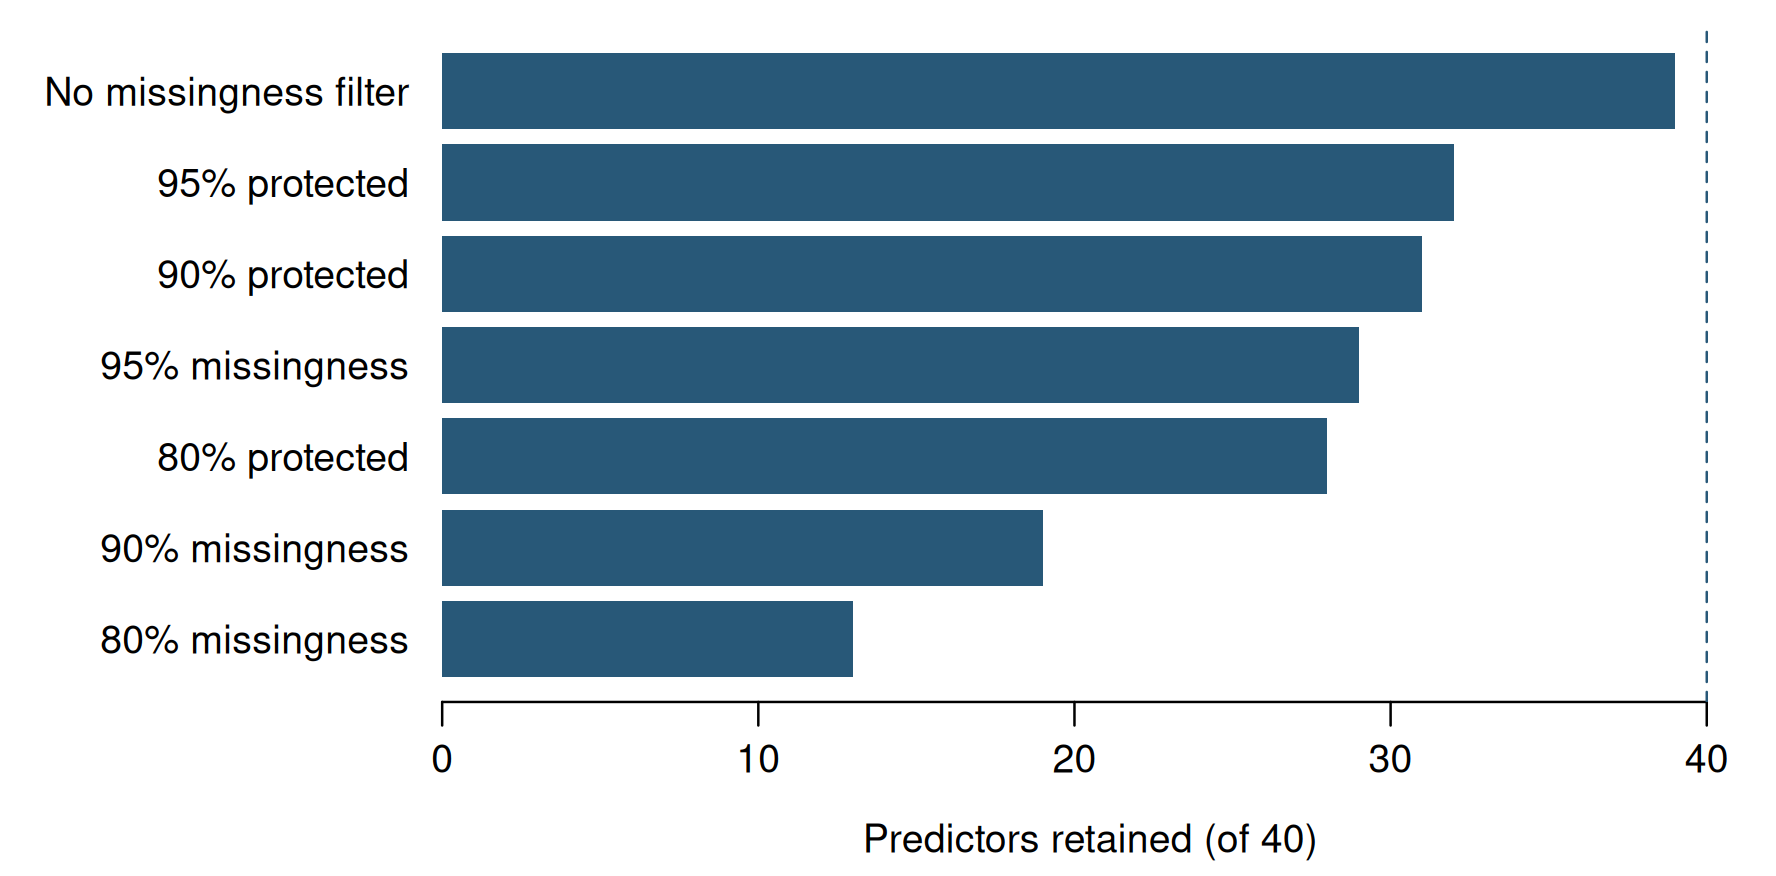
\includegraphics[width=0.84\linewidth,height=0.27\textheight,keepaspectratio]{images/feature_retention.png}
	\caption{Number of retained predictors in each feature-selection
		alternative.}\label{fig:chapter4-3}
\end{figure}

Under the 80\% missingness-only threshold, 13 of 40 predictors
remained, representing a 67.5\% reduction in the predictor
count. The matched rule-based clinical-review configuration retained
28 predictors. The corresponding serialised CSV reductions
relative to the rewritten CSV baseline were 34.02\%
and 14.28\%, respectively. At the 90\% threshold the standard
and review configurations retained 19 and 31 predictors, while at 95\%
they retained 29 and 32. Thus, more aggressive filtering reduced data
dimensions and serialised size more strongly but excluded more clinical
variables.

The rule-based clinical-protection configurations retained more
predictors than the corresponding missingness-only alternatives,
including the explicitly protected Lactate variable. The term clinical
review in the configuration names denotes these predefined rules; it
does not imply an independent assessment by clinicians. Changes in the
number of columns were not proportional to changes in file size. For
example, retaining 13 rather than 40 predictors reduced dimensionality
by 67.5\%, but reduced the standardised serialised CSV size by 34.02\%.
Structural columns, the values of retained variables and serialisation
overhead continued to contribute to the file.

For the feature-selection comparisons, percentage reductions in
serialised size were calculated relative to the standardised rewritten
CSV of 77,550,287 bytes. This common denominator removes size
differences caused solely by rewriting the CSV. The original source file
of 75,688,701 bytes is retained as the reference for the separate
baseline compression experiment. The distinction is necessary when
comparing percentage reductions across the two stages.

\section{Phase Four: Principal Component Analysis and Autoencoder
	Reduction}\label{phase-four-principal-component-analysis-and-autoencoder-reduction}

PCA and an autoencoder were applied to the original and selected
numerical feature sets with target latent dimensions of 2, 4, 8 and 16,
subject to the number of usable input features. Unlike lossless CSV,
gzip or Parquet, these methods produce transformed representations that
may not reproduce the original observed values exactly. Their
performance was therefore examined using both representation size and
reconstructed-value preservation.

\begin{longtable}[]{@{}
		>{\raggedright\arraybackslash}p{\dimexpr 0.2000\textwidth - 2\tabcolsep\relax}
		>{\raggedright\arraybackslash}p{\dimexpr 0.2000\textwidth - 2\tabcolsep\relax}
		>{\raggedright\arraybackslash}p{\dimexpr 0.2000\textwidth - 2\tabcolsep\relax}
		>{\raggedright\arraybackslash}p{\dimexpr 0.2000\textwidth - 2\tabcolsep\relax}
		>{\raggedright\arraybackslash}p{\dimexpr 0.2000\textwidth - 2\tabcolsep\relax}@{}}
	\caption{Reconstruction accuracy on the original feature set.}\label{tab:chapter4-5}\\
	\toprule\noalign{}
	\textbf{k} & \textbf{PCA observed \(R^2\)} & \textbf{PCA 5-NN overlap} & \textbf{AE observed \(R^2\)} & \textbf{AE 5-NN overlap} \\
	\midrule\noalign{}
	\endfirsthead
	\toprule\noalign{}
	\textbf{k} & \textbf{PCA observed \(R^2\)} & \textbf{PCA 5-NN overlap} & \textbf{AE observed \(R^2\)} & \textbf{AE 5-NN overlap} \\
	\midrule\noalign{}
	\endhead
	\bottomrule\noalign{}
	\endlastfoot
	2 & 0.259 & 0.205 & 0.444 & 0.306 \\
	4 & 0.345 & 0.226 & 0.589 & 0.442 \\
	8 & 0.548 & 0.359 & 0.815 & 0.717 \\
	16 & 0.676 & 0.436 & 0.907 & 0.771 \\
\end{longtable}

\begin{figure}
	\centering
	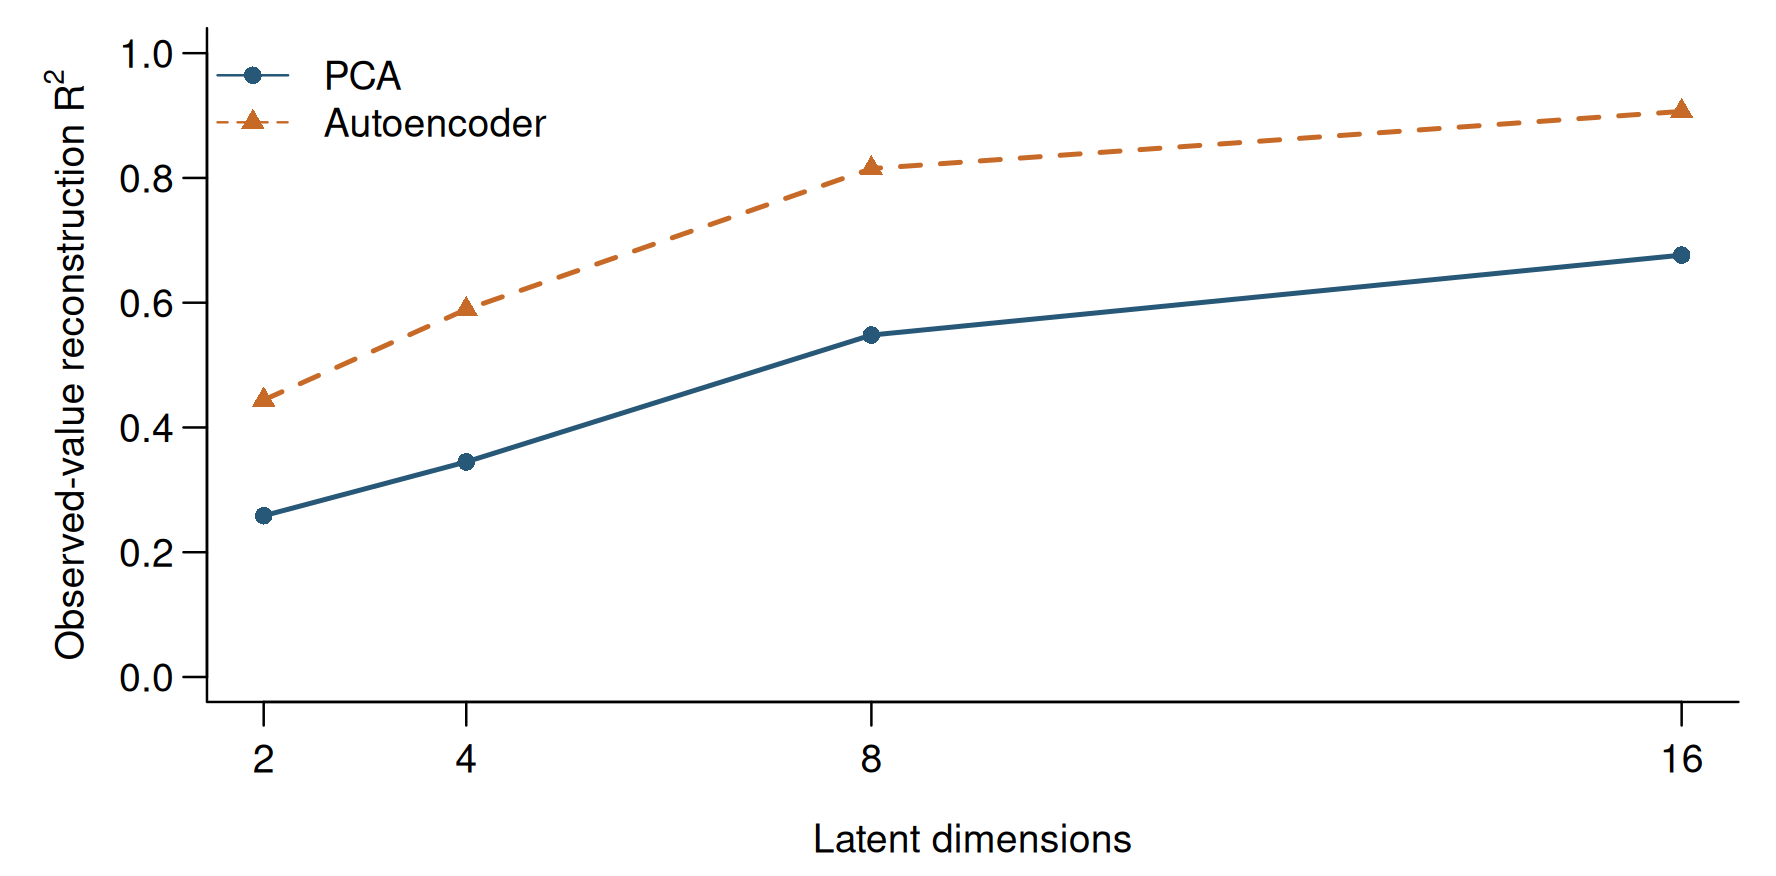
\includegraphics[width=0.84\linewidth,height=0.27\textheight,keepaspectratio]{images/reconstruction_r2.png}
	\caption{Reconstructed observed-value R-squared for PCA and autoencoder
		on the original feature set.}\label{fig:chapter4-4}
\end{figure}

On the original numerical feature set, the autoencoder obtained a higher
standardised observed-value reconstruction \(R^2\) than PCA at each target
dimension. At two components, the values were 0.444 for the autoencoder
and 0.259 for PCA. With 16 components, they increased to 0.907 and
0.676, respectively. In general, increasing latent dimensionality
improved reconstruction, while also increasing the size of the
transmitted representation. Autoencoder fitting required substantially
more computation than PCA fitting, establishing a trade-off between
reconstruction quality and preparation cost.

Reconstruction \(R^2\) was calculated from squared errors on originally
observed values after standardisation. This measure differs from the
intrinsic explained-variance ratio of a fitted PCA model. Reconstruction
results for different feature-selected datasets must also be interpreted
with care because the number and identity of the retained input features
differ. The analysis therefore considers retention of original
observations separately from the reconstruction accuracy of values that
remained in each representation.

\noindent The original feature set admitted all four widths. Selection reduced the number of available numerical fields, so the same choices were not feasible throughout the experiment.

\subsection{Feasible latent dimensionalities}\label{feasible-latent-dimensionalities}

The feasible number of latent dimensions depended on the varying
numerical features available after selection. In the 80\%
missingness-only dataset, PCA and autoencoder representations could be
formed at two and four components, whereas eight- and sixteen-component
representations were not available. In the 90\% missingness-only
dataset, two, four and eight components were available, but sixteen were
not. These restrictions excluded six method-by-dimension combinations
from the 88 combinations defined by the full design, leaving 82 feasible
packages for evaluation. Subsequent comparisons include only
representations that could be constructed.

\section{Phase Five: Descriptive Information-Preservation
	Checks}\label{phase-five-descriptive-information-preservation-checks}

Information preservation was examined through numerical reconstruction
and the retention of local sample-neighbourhood relationships. A random
sample of up to 200 patients, using one hourly record for each sampled
patient, was used to calculate overlap in the five- and
ten-nearest-neighbour sets before and after reconstruction. Distances
were calculated on consistently scaled original-feature values.
Neighbourhood relationships measured directly in latent coordinates were
treated as descriptive because PCA and autoencoder coordinate scales are
not equivalent.

On the original feature set, the mean five-nearest-neighbour overlap
increased from 0.205 to 0.436 as PCA dimensionality increased from two
to sixteen components. For autoencoders, it increased from 0.306 to
0.771 over the same range. The results indicate that higher-dimensional
reconstructions generally retained more of the local similarity
structure in the sampled records. Nearest-neighbour overlap and
reconstruction \(R^2\) nevertheless describe numerical properties of the data
rather than validated effects on a clinical research task.

An additional plausibility assessment counted reconstructed values that
fell outside predefined numerical ranges when the original observed
values were within those ranges. On the original feature set at eight
latent components, the autoencoder produced 54,805 newly flagged
instances, compared with 10,179 for PCA. The count did not vary
monotonically with the number of components. This finding is important
because a high aggregate reconstruction \(R^2\) may coexist with notable
errors in particular variables. The bounds used for this assessment were
exploratory screening limits, rather than clinically validated
acceptance thresholds.

Information loss from feature selection differs from reconstruction
error. A column excluded before compression is absent from every
subsequently transmitted representation, even when the resulting file is
preserved without numerical alteration. Thus, exact recovery of a
selected-column package establishes fidelity to the selected dataset,
not completeness relative to the source. Both retained measurement
coverage and reconstruction accuracy are needed to understand the
trade-offs associated with reduced representations.

\section{Phase Six: Packaging, Network Delivery and Receiver
	Reconstruction}\label{phase-six-packaging-network-delivery-and-receiver-reconstruction}

Packaging and delivery experiments combined the original and
feature-selected datasets with lossless encodings and PCA or autoencoder
representations. Eighty-two feasible packages were examined under two
delivery-cost scenarios, yielding 164 package-scenario comparisons.
Across the package experiments, 586 authenticated SSH/SCP trials
completed successfully, with SHA-256 verification at the university
receiver. The received packages also passed the configured remote
recovery checks. Under the adaptive repetition policy, 56 packages were
transferred ten times and 26 packages once, so precision of the
transfer-time estimates varied between package types.

Transfer and recovery measurements were collected over multiple
measurement sessions. Because network throughput and server workload may
change over time, variations in the observed durations cannot be
attributed exclusively to the compression method or payload size. This
variability is considered when interpreting rankings based on delivery
time.

At the receiving node, the transferred archive was checked, unpacked and
decoded or decompressed; the recovered output was also persisted where
required by the representation. The reported end-to-end delivery
estimate combines separately timed preparation, package handling,
network transfer, integrity checking and receiver-side recovery stages.
It is therefore an additive cost measure rather than a single
synchronised wall-clock interval. The more limited Phase Two comparison
includes only baseline packaging and SCP time.

Two delivery scenarios were evaluated. The existing-payload scenario
assumes that the encoded dataset or compressed file has already been
created; it includes package handling, network delivery and recovery but
excludes initial fitting and encoding costs. The fresh-data scenario
additionally includes model fitting, encoding and initial payload
creation, with a model-reuse count of one. Both scenarios exclude
initial source-data loading, general preprocessing and feature
selection. Their estimates therefore represent defined parts of the
transfer workflow, rather than the cost of every operation in a
production data system.

\begin{longtable}[]{@{}
		>{\raggedright\arraybackslash}p{\dimexpr 0.175\textwidth - 2\tabcolsep\relax}
		>{\raggedright\arraybackslash}p{\dimexpr 0.1584\textwidth - 2\tabcolsep\relax}
		>{\raggedright\arraybackslash}p{\dimexpr 0.1667\textwidth - 2\tabcolsep\relax}
		>{\raggedright\arraybackslash}p{\dimexpr 0.1667\textwidth - 2\tabcolsep\relax}
		>{\raggedright\arraybackslash}p{\dimexpr 0.1667\textwidth - 2\tabcolsep\relax}
		>{\raggedright\arraybackslash}p{\dimexpr 0.1667\textwidth - 2\tabcolsep\relax}@{}}
	\caption{Original feature set: transmitted size and scoped delivery costs.}\label{tab:chapter4-6}\\
	\toprule\noalign{}
	\textbf{Package} & \textbf{Sent MB} & \textbf{SCP (s)} & \textbf{Existing (s)} & \textbf{Initial prep (s)} & \textbf{Fresh (s)} \\
	\midrule\noalign{}
	\endfirsthead
	\toprule\noalign{}
	\textbf{Package} & \textbf{Sent MB} & \textbf{SCP (s)} & \textbf{Existing (s)} & \textbf{Initial prep (s)} & \textbf{Fresh (s)} \\
	\midrule\noalign{}
	\endhead
	\bottomrule\noalign{}
	\endlastfoot
	AE 2 & 6.85 & 20.76 & 36.66 & 613.01 & 649.67 \\
	AE 4 & 12.11 & 12.42 & 28.71 & 456.45 & 485.16 \\
	AE 8 & 22.73 & 14.32 & 31.83 & 436.46 & 468.30 \\
	AE 16 & 42.91 & 34.38 & 56.51 & 334.28 & 390.79 \\
	GZIP & 14.54 & 14.38 & 22.79 & 4.37 & 27.16 \\
	PARQUET & 7.61 & 8.71 & 28.67 & 1.05 & 29.72 \\
	PCA 2 & 7.32 & 5.63 & 21.41 & 3.74 & 25.15 \\
	PCA 4 & 12.90 & 11.09 & 26.90 & 3.33 & 30.23 \\
	PCA 8 & 24.07 & 19.84 & 41.79 & 5.38 & 47.17 \\
	PCA 16 & 46.39 & 50.85 & 70.57 & 4.73 & 75.30 \\
	ZSTD & 14.73 & 40.03 & 47.70 & 0.49 & 48.18 \\
\end{longtable}

\begin{figure}
	\centering
	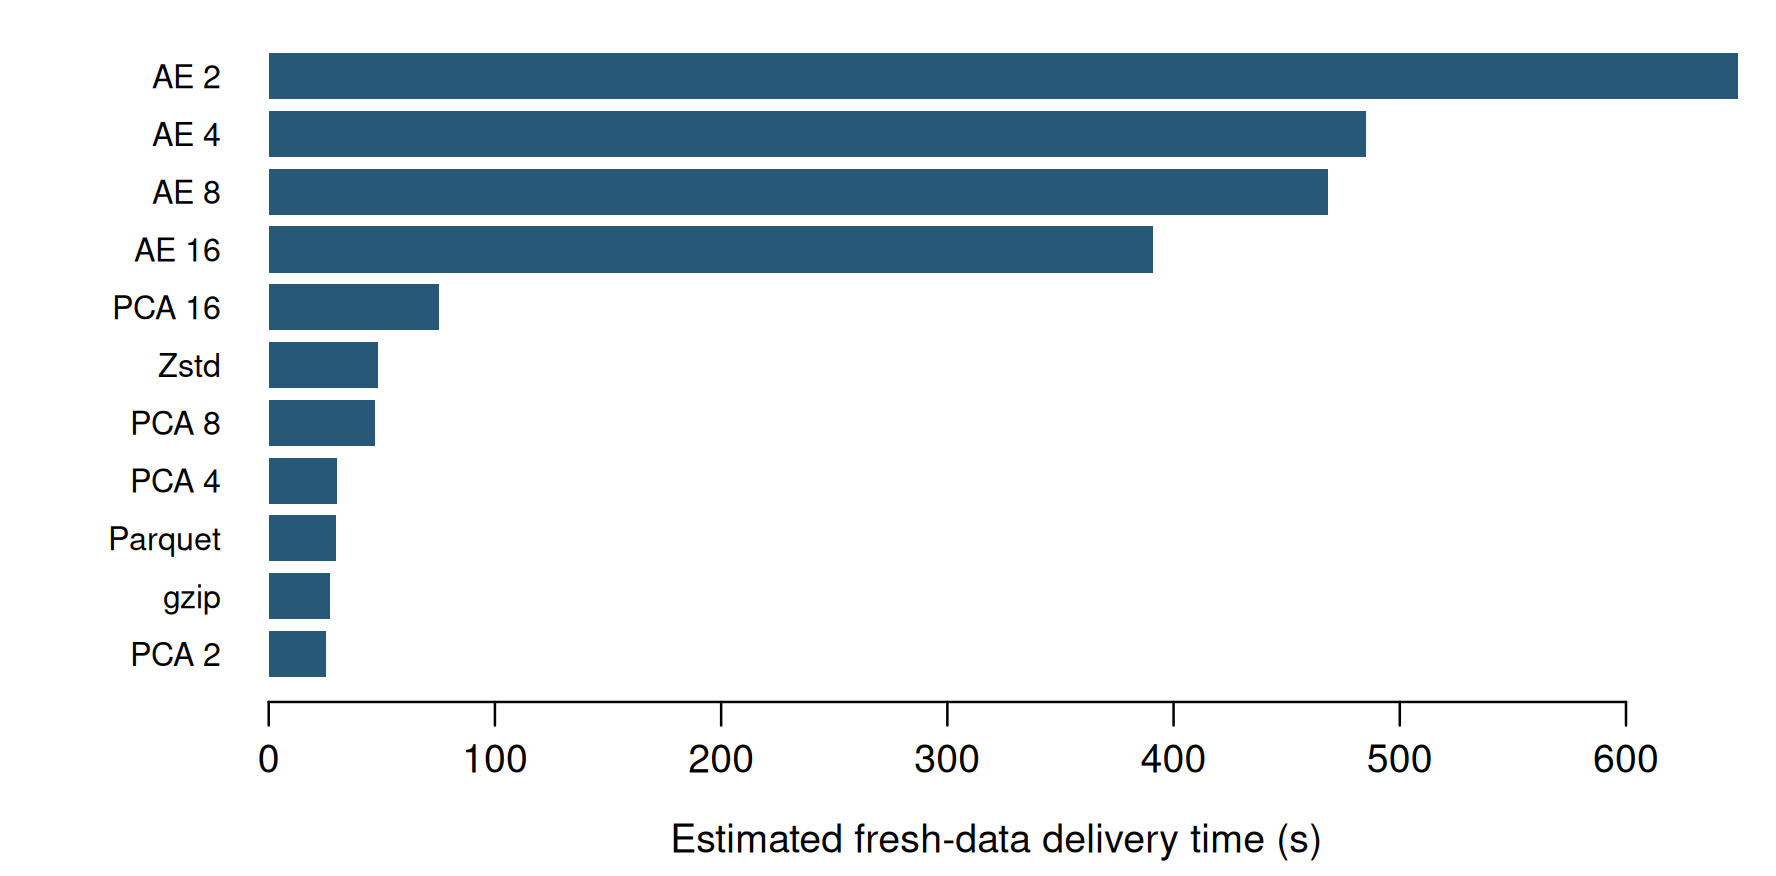
\includegraphics[width=0.84\linewidth,height=0.27\textheight,keepaspectratio]{images/fresh_data_times.png}
	\caption{Estimated delivery time for fresh data on the original feature set, with fitting charged to one delivery where applicable.}\label{fig:chapter4-5}
\end{figure}

A comparison of two-component PCA and autoencoder representations shows
the effect of preparation overhead. The autoencoder package transmitted
6.85 MB, slightly less than the 7.32 MB PCA package. Its fresh-data
delivery estimate was nevertheless 649.67 s, compared with 25.15 s for
PCA, primarily because autoencoder fitting accounted for 609.48 s. Under
the existing-payload scenario, the corresponding estimates were 36.66 s
and 21.41 s. The results indicate that reducing the transmitted bytes
does not necessarily minimise the time required to prepare, deliver and
recover the data.

Among the lossless methods applied to the original feature set, the
fresh-data delivery estimates were 27.16 s for gzip, 29.72 s for Parquet
and 48.18 s for Zstandard. Parquet had the shortest baseline
preparation-plus-SCP time in Phase Two, but the more comprehensive
delivery estimates differed because they also included package handling,
integrity verification and recovery at the receiving server. The
difference demonstrates the importance of defining the stages included
in a performance measure before comparing transfer strategies.

\section{Multi-Criteria Decision
	Analysis}\label{multi-criteria-decision-analysis}

The Technique for Order Preference by Similarity to Ideal Solution
(TOPSIS) was used to assess transfer alternatives under explicit
fidelity and preparation requirements. The primary analysis assigned
equal weights of 1/7 (14.2857\%) to transmitted bytes, effective
delivery time, standardised observed-value reconstruction \(R^2\),
five-nearest-neighbour overlap, clinical-predictor retention, retained
original measurements and newly flagged clinical-range violations. The
first two criteria and range violations were minimised, while the other
four were maximised. Balanced, transfer-priority and utility-priority
weight profiles were also examined to assess ranking sensitivity.

Alternatives were ranked within three preservation requirements: exact
delivery of the complete source, exact delivery of selected columns, and
delivery allowing some reconstruction loss. These categories represent
different practical needs and are not interchangeable. In particular, a
lossless file containing selected columns retains the data in those
columns but cannot restore columns previously excluded by feature
selection. TOPSIS ranks alternatives against the criteria and weights
defined for each comparison; it does not establish clinical suitability
by itself.

\begin{longtable}[]{@{}lll@{}}
	\caption{First-ranked strategies with equal TOPSIS weights in the loss-tolerant scenario.}\label{tab:chapter4-7}\\
	\toprule\noalign{}
	\textbf{Feature set} & \textbf{Existing payload} & \textbf{Fresh data} \\
	\midrule\noalign{}
	\endfirsthead
	\toprule\noalign{}
	\textbf{Feature set} & \textbf{Existing payload} & \textbf{Fresh data} \\
	\midrule\noalign{}
	\endhead
	\bottomrule\noalign{}
	\endlastfoot
	original & PARQUET (0.952) & PARQUET (0.991) \\
	00 no missingness filter & PARQUET (0.951) & PARQUET (0.995) \\
	80 missingness & PARQUET (0.927) & PARQUET (0.993) \\
	80 clinical review & GZIP (0.923) & PARQUET (0.989) \\
	90 missingness & PARQUET (0.937) & PARQUET (0.997) \\
	90 clinical review & GZIP (0.923) & PARQUET (0.990) \\
	95 missingness & PARQUET (0.923) & PARQUET (0.994) \\
	95 clinical review & ZSTD (0.908) & PARQUET (0.986) \\
\end{longtable}

For fresh data, Parquet ranked first in all eight
dataset groups under the equal-weight, loss-tolerant comparison. The
choice varied when the payload already existed. Gzip ranked
first for the 80\% and 90\% rule-based clinical-review sets, Zstandard
for the 95\% rule-based review set, and Parquet for the other groups.
Under the transfer-priority sensitivity profile, the 95\%
clinical-review existing-payload comparison instead selected the
two-component autoencoder, illustrating how rankings depend on
the relative importance assigned to transfer and fidelity measures.

The seven-criterion package rankings in this chapter use SCP delivery measurements for the 82 configurations. The rsync observations cover the five baseline files and three prepared archives. They support the separate Phase Two format ranking and the archive comparisons reported here. A seven-criterion rsync ranking for the full set would require verified rsync timings for the other configurations.

TOPSIS scores are relative to the candidates considered in each ranking
group. The score assigned to a particular feature set cannot therefore
be interpreted as a direct measure of clinical usefulness relative to a
different feature set. Sensitivity analysis further showed that applying
a zero-new-violation threshold restricted each group to lossless
alternatives, for which Parquet ranked first under equal weights. When
the exploratory range-screen threshold was relaxed, additional
candidates became eligible and selected rankings changed, including
selection of gzip in the 90\% clinical-review existing-payload group at
a 1\% threshold. These thresholds indicate the response of the ranking
to selection rules rather than medically established safety boundaries.

\section{Verified delivery with SCP and rsync}\label{sec:paired-results}
All 24 uninterrupted deliveries passed remote verification on the first attempt. All eight deliberately interrupted deliveries passed on the second attempt. The 32 deliveries therefore accounted for 40 attempts. Table~\ref{tab:paired-transport} gives the time to verified publication of each prepared archive.

\begin{table}[htbp]
\centering
\caption{Time to verified publication on the KNUST route. Each row represents four matched pairs.}\label{tab:paired-transport}
\begin{tabular}{@{}llrrr@{}}
\toprule
Archive & Condition & Median SCP & Median rsync & Paired difference \\
 & & (s) & (s) & (s) \\
\midrule
Parquet & Uninterrupted & 7.87 & 9.19 & $+1.09$ \\
gzip & Uninterrupted & 9.34 & 11.31 & $+0.46$ \\
AE-16 & Uninterrupted & 21.54 & 21.35 & $-1.06$ \\
AE-16 & Interrupted & 35.66 & 25.43 & $-10.46$ \\
\bottomrule
\end{tabular}
\end{table}

A negative paired difference means rsync finished sooner. The last column is the median of the within-block differences. For the uninterrupted 7.61 MB Parquet and 14.54 MB gzip archives, SCP finished sooner in three and four blocks respectively. For the uninterrupted 42.91 MB AE-16 archive, rsync finished sooner in three blocks. After interruption, rsync finished sooner in all four, with savings ranging from 7.66 to 13.89 seconds. Both transports recovered every interrupted delivery. Their difference lay in the time needed to finish.

% !TeX root = thesis.tex
\section{Discussion of the findings}\label{sec:discussion}
\noindent For the receiving research team, a successful copy answers only the first question. The practical choice also depends on which measurements survive, how soon the table can be read and what happens if the connection breaks.

\subsection{What is lost when a column is removed?}
Missingness reached 65.05\% across the cohort, but it varied considerably by measurement. Heart rate was available in most hourly records, whereas lactate was missing from 96.57\%. Removing lactate would therefore remove a relatively small number of values, yet those values would be lost to any researcher interested in the occasions when lactate was measured. This is a concrete difficulty with applying a single missingness rule to a clinical record. The profiling results in Table~\ref{tab:chapter4-1} give the receiving team a basis for deciding which omissions it can accept.

At the 80\% missingness threshold, filtering alone retained 13 of 40 predictors. With the protection rules, 28 remained. The first choice saved more space, while the second preserved more measurements. The rules were exploratory and received no independent clinical endorsement. Likewise, a high correlation between two variables warranted review of what each measured before either was dropped. This extends the preprocessing question raised by \citet{Tang2020}: for a transfer, the analyst also needs a record of what the sender left out.

\subsection{Which costs matter to the receiver?}
At 16 components, the autoencoder recovered more of the variation in observed values than PCA. Its five-nearest-neighbour overlap was also higher, 0.771 against 0.436 on the original feature set. This finding is consistent with the ability of nonlinear encoders to learn compact representations described by \citet{Hinton2006}. An overall improvement can nevertheless conceal errors in individual measurements. At eight components, for instance, the autoencoder produced 54,805 newly flagged range violations against 10,179 for PCA. These are exploratory numerical screens. The ECG evaluation by \citet{Guan2026} illustrates a further test. The analyst can repeat the intended analysis on the recovered records. For this cohort, whether the reconstructions preserve performance on a patient-level task remains open.

For a research unit receiving a fresh extract, the sender's time matters. At two components, the autoencoder archive occupied 6.85 MB against 7.32 MB for PCA, yet their fresh-data delivery estimates were 649.67 s and 25.15 s respectively. Fitting alone took 609.48 s for that autoencoder. When the payloads already existed, their corresponding delivery estimates fell to 36.66 s and 21.41 s. A team choosing between those methods should first establish whether the payload will be created specifically for the delivery.

The columnar storage comparisons of \citet{Zeng2023} and \citet{Liu2025} describe trade-offs between size and processing cost. The KNUST results show how the choice of endpoint affects the practical recommendation. Parquet ranked first in the eight equal-weight, loss-tolerant fresh-data groups. Yet on the original feature set gzip had a shorter estimated fresh-data delivery time than Parquet, 27.16 s against 29.72 s. The ranking also rewarded small packages and information preservation, so a team concerned chiefly with elapsed time can reasonably make a different choice.

The direct transfers of the five Phase Two files help distinguish the effect of the representation from that of the transport. Switching from the source CSV to Parquet reduced the median copy time with either method. For Parquet itself, the median within-block difference in copy time was only 0.13 s. Across the four blocks, each method copied Parquet sooner twice. The receiving team has a clearer basis here for choosing a smaller lossless representation than for preferring one transport for every uninterrupted upload.

\subsection{What happens when an upload stops?}
The 586 successful baseline package transfers established that data could reach the university server and be recovered there. Every one completed on its first attempt. The follow-up supplied the missing recovery evidence. On the uninterrupted link, the smaller lossless archives generally reached verified publication sooner with SCP. After the break in the AE-16 upload, both methods succeeded on their first retry, but rsync finished sooner in each paired block.

The sender's copy traces help explain the difference. SCP forwarded 42.91 MB on each successful retry, approximately the size of the whole archive. Rsync forwarded between 23.07 and 23.37 MB. This pattern is consistent with the reuse of matching blocks at the receiver described by \citet{TridgellMackerras1996}. These byte counts describe the outgoing copy protocol before SSH encryption. Over the four interrupted pairs the median time saving with rsync was 10.46 s. The finding supports retaining a partial copy for a retry on a comparable route, especially when preparing the archive has already taken considerable time.

\subsection{Scope of the evidence}
The study used one public cohort and one route to KNUST. The original timing policy produced ten observations for some packages and one for others. The paired archive experiment occupied a single ten-minute window. The paired baseline files were transferred on a different day. Comparisons within each block limit the effect of changes between blocks, although the link can also change between successive transfers. Only AE-16 was deliberately interrupted, at one point in the upload. Other file sizes, outage durations, server loads and hospital links in Ghana could give different timings.

The original delivery estimates add separately measured stages and exclude initial data loading, general preprocessing, feature selection and production ingestion. The paired experiments timed the transfer of files already prepared at the sender and their verified publication. The study did not assess routine service availability or performance at other institutions. Neighbourhood comparisons used one record from each of at most 200 sampled patients. No downstream predictive task or clinician assessment established that a reduced representation was suitable for patient care.


\section{Chapter Summary}\label{sec:results-summary}
Parquet offered the strongest lossless baseline for this cohort. Where approximate recovery was acceptable, the choice also depended on which measurements the receiver needed and whether the sender had already fitted the model. Both SCP and rsync completed every interrupted archive delivery, with rsync reaching verification sooner in all four interrupted pairs. Chapter~\ref{conclusion} draws on these findings to make recommendations for research data transfers.
